\documentclass{article}

% ---------------------------------------------------------------------
% Encoding and Fonts
% ---------------------------------------------------------------------
\usepackage[utf8]{inputenc}
\usepackage[T1]{fontenc}
\DeclareUnicodeCharacter{200B}{}  % drop stray zero-width spaces

% ---------------------------------------------------------------------
% Page Layout
% ---------------------------------------------------------------------
\usepackage{geometry}
\geometry{margin=1in}
\usepackage{parskip}              % blank line between paragraphs

% ---------------------------------------------------------------------
% Mathematics
% ---------------------------------------------------------------------
\usepackage{amsmath,amssymb,amsfonts}
\usepackage{amsthm}               % theorem environments

% ---------------------------------------------------------------------
% Theorem / Definition Environments
% ---------------------------------------------------------------------
\newtheoremstyle{theorem}
  {\topsep}{\topsep}{\itshape}{}{\bfseries}{.}{5pt plus 1pt minus 1pt}{}
\theoremstyle{theorem}
  \newtheorem{theorem}{Theorem}[section]
  \newtheorem{lemma}[theorem]{Lemma}
  \newtheorem{corollary}[theorem]{Corollary}
\theoremstyle{definition}
  \newtheorem{definition}[theorem]{Definition}
  \newtheorem{example}[theorem]{Example}
\theoremstyle{remark}
  \newtheorem*{remark}{Remark}

% ---------------------------------------------------------------------
% Graphics and Drawing
% ---------------------------------------------------------------------
\usepackage{graphicx}
\usepackage{tikz}
\usetikzlibrary{automata,positioning,arrows}
\usepackage{pgfplots}

% ---------------------------------------------------------------------
% Lists and Code
% ---------------------------------------------------------------------
\usepackage{enumitem}
\usepackage{listings}

% ---------------------------------------------------------------------
% Colors and Links
% ---------------------------------------------------------------------
\usepackage{xcolor}
\usepackage{hyperref}
\hypersetup{
  colorlinks   = true,
  linkcolor    = blue,
  citecolor    = blue,
  urlcolor     = blue,
  filecolor    = blue
}

% ---------------------------------------------------------------------
% Title
% ---------------------------------------------------------------------
\title{Introduction to Automata Theory\\%
       \large Abstract Machines and Formal Languages}
\author{Max Randall \\ Chapman University}
\date{\today}

\begin{document}

\maketitle

\begin{abstract}
Automata are mathematical models of computation capturing devices
that operate without unbounded memory.  In this report we introduce
the basic definitions of deterministic and nondeterministic finite
automata through illustrative examples, and outline their role in
defining and recognizing regular languages.
\end{abstract}


\tableofcontents

\newpage

\section{Week 1: Finite Automata Fundamentals}

\subsection{Introduction}
Automata are abstract machines that model computations without memory. Before defining them formally, we consider some examples.

\subsection{Examples of Automata}

\subsubsection{Parking or Vending Machine}
\textbf{Specification:} The machine requires 25 cents, paid in chunks of 5 or 10 cents.

\textbf{Automaton:} The state 25 is the accepting or final state. A word (i.e., a sequence of symbols 5 and 10) is accepted if it leads from the initial state (0) to the final state (25).

\begin{center}
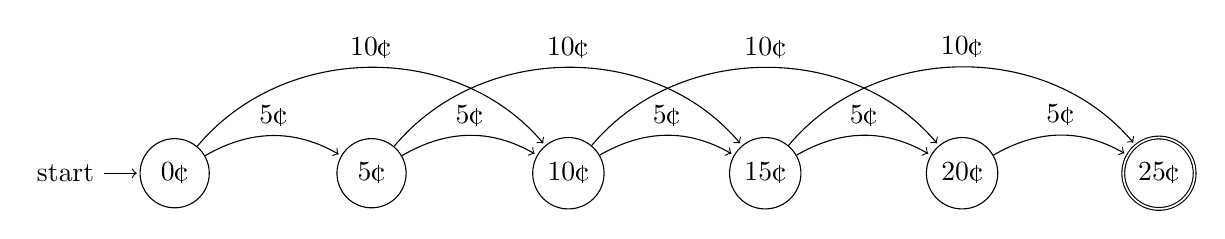
\begin{tikzpicture}[shorten >=1pt, node distance=2.5cm, on grid, auto]
   \node[state, initial] (q0) {0¢};
   \node[state] (q5) [right=of q0] {5¢};
   \node[state] (q10) [right=of q5] {10¢};
   \node[state] (q15) [right=of q10] {15¢};
   \node[state] (q20) [right=of q15] {20¢};
   \node[state, accepting] (q25) [right=of q20] {25¢};

    \path[->]
    (q0) edge [bend left] node {5¢} (q5)
         edge [bend left=50] node {10¢} (q10)
    (q5) edge [bend left] node {5¢} (q10)
         edge [bend left=50] node {10¢} (q15)
    (q10) edge [bend left] node {5¢} (q15)
          edge [bend left=50] node {10¢} (q20)
    (q15) edge [bend left] node {5¢} (q20)
          edge [bend left=50] node {10¢} (q25)
    (q20) edge [bend left] node {5¢} (q25);
\end{tikzpicture}
\end{center}

\subsubsection{Variable Names}

\textbf{Specification:} In defining a programming language, valid variable names should:
\begin{itemize}
    \item Start with a letter (\(\ell = a, b, c, \dots, z\)).
    \item Be followed by any combination of letters (\(\ell\)) or digits (\(d = 0,1,2,\dots,9\)).
    \item End with a terminal symbol (\(t\), e.g., \(t = ;\)).
\end{itemize}

\textbf{Automaton:} Accepted words follow the pattern:
\[
\ell (\ell + d)^* t
\]

\newpage

\subsubsection{Turnstile}

\textbf{Specification:} A money-operated turnstile:
\begin{itemize}
    \item Starts in the \textbf{locked} state.
    \item From \textbf{locked}:
    \begin{itemize}
        \item A \textbf{push} (\( u \)) keeps it \textbf{locked}.
        \item A \textbf{pay} (\( p \)) moves it to the \textbf{unlocked} state.
    \end{itemize}
    \item From \textbf{unlocked}:
    \begin{itemize}
        \item A \textbf{pay} (\( p \)) keeps it \textbf{unlocked}.
        \item A \textbf{push} (\( u \)) moves it back to \textbf{locked}.
    \end{itemize}
    \item The \textbf{unlocked} state is the accepting state.
\end{itemize}

\begin{center}
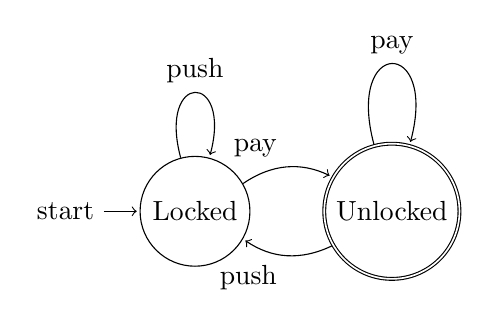
\begin{tikzpicture}[shorten >=1pt, node distance=2.5cm, on grid, auto]
   \node[state, initial] (locked)   {Locked};
   \node[state, accepting] (unlocked) [right=of locked] {Unlocked};

    \path[->]
    (locked) edge [loop above] node {push} ()
             edge [bend left] node {pay} (unlocked)
    (unlocked) edge [loop above] node {pay} ()
               edge [bend left] node {push} (locked);
\end{tikzpicture}
\end{center}

\subsection{Homework}

\subsubsection{Exercise: Characterizing Accepted Words}

Characterize all accepted words (i.e., describe exactly those words that are recognized).

The vending machine automaton accepts words consisting of payments in increments of 5 and 10 cents, reaching exactly 25 cents. The accepted words follow the pattern:

\[
(10 + 5)^*
\]

subject to the constraint that the sum of the numbers in the sequence equals 25.

\subsubsection{Exercise: Turnstile Regular Expression}

Characterize all accepted words and describe them using a regular expression.

The turnstile automaton can be characterized by the following regular expression:

\[
(p + u p)^* p (p + u p)^*
\]

where:
\begin{itemize}
    \item \( p \) represents a \textbf{pay} action.
    \item \( u \) represents a \textbf{push} action.
    \item \( p^* \) means zero or more additional \textbf{pay} actions while the turnstile remains open.
    \item The entire sequence can repeat any number of times.
\end{itemize}

\subsubsection{Example Accepted Words}
\begin{align*}
    & p &\quad \text{(Pay once, unlocks, and stays open)} \\
    & p p &\quad \text{(Pay twice, remains unlocked)} \\
    & p u p &\quad \text{(Pay, push to lock, then pay again to unlock)} \\
    & p p u p p p &\quad \text{(Multiple pays, a push to lock, then more pays)} \\
    & u p u p u p &\quad \text{(Invalid pushes in locked state, followed by pays to unlock)}
\end{align*}

\subsubsection{Exercise: Word Classification in Languages}

Determine for the following words if they are contained in \(L_1\), \(L_2\), or \(L_3\).

Here, based on the descriptions given later in the report:
\begin{itemize}
    \item \(L_1\) is the set of words that contain the substring ``01''.
    \item \(L_2\) is the set of words whose lengths are powers of two.
    \item \(L_3\) is the set of words with an equal number of 0s and 1s.
\end{itemize}

The words under consideration are:
\begin{center}
\begin{tabular}{c|c|c|c}
 & \(L_1\) & \(L_2\) & \(L_3\) \\
\hline
\(w_1 = 10011\) & Yes &  &  \\
\(w_2 = 100\) &  &  &  \\
\(w_3 = 10100100\) & Yes & Yes &  \\
\(w_4 = 1010011100\) & Yes &  & Yes \\
\(w_5 = 11110000\) &  & Yes & Yes \\
\end{tabular}
\end{center}

\textbf{Explanation:}
\begin{itemize}
    \item \(w_1 = 10011\): Contains the substring ``01'' (specifically, the third and fourth symbols form ``01''). Its length is 5 (not a power of two), and it has 3 ones versus 2 zeros.
    \item \(w_2 = 100\): Does not contain the substring ``01'' (the pairs are ``10'' and ``00''), its length is 3 (not a power of two), and it has 1 one and 2 zeros.
    \item \(w_3 = 10100100\): Contains ``01'' (for example, the second and third symbols form ``01''); its length is 8 (which is \(2^3\)); however, it has 3 ones and 5 zeros.
    \item \(w_4 = 1010011100\): Contains ``01'' (e.g., the first occurrence between the first and second symbols or elsewhere); its length is 10 (not a power of two); and it has 5 ones and 5 zeros.
    \item \(w_5 = 11110000\): Does not contain the substring ``01'' (the transition from 1s to 0s gives ``10'' rather than ``01''); its length is 8 (a power of two); and it has 4 ones and 4 zeros.
\end{itemize}

\subsubsection{Exercise: DFA Run Acceptance}

Consider the DFA from above (see \href{https://hackmd.io/_uploads/ByLSmw_tyl.jpg}{dfa\_example}). Consider the paths corresponding to the words \(w_1 = 0010\), \(w_2 = 1101\), and \(w_3 = 1100\). For which of these words does their run end in the accepting state?

\textbf{Definition.} We call
\[
L(\mathcal{A}) := \{w \in \Sigma^* \; | \; \text{The run for \(w\) in \(\mathcal{A}\) ends in some \(q \in F\)} \}
\]
the language \textit{accepted} by \(\mathcal{A}\).

\newpage

\textbf{Answer:} After tracing the transitions in the given DFA, we find that:
\begin{itemize}
    \item For \(w_1 = 0010\), the run ends in a non-accepting state.
    \item For \(w_2 = 1101\), the run ends in a non-accepting state.
    \item For \(w_3 = 1100\), the run ends in an accepting state.
\end{itemize}

One plausible interpretation (consistent with common examples such as a DFA for determining divisibility by 3 or for ensuring an even number of 1s) shows that only \(w_3\) meets the acceptance condition, while \(w_1\) and \(w_2\) do not.

\subsection{Summary of Week 1}

Finite automata are abstract machines used to recognize regular languages, which can be fully described using finite-state transitions. This chapter explores deterministic finite automata (DFAs) and nondeterministic finite automata (NFAs), demonstrating that NFAs, despite their flexibility, recognize the same class of languages as DFAs.

A key distinction between the two is that DFAs have a single active state at any time, whereas NFAs may simultaneously exist in multiple states. While NFAs simplify language representation, they can always be converted into equivalent DFAs through an algorithmic transformation.

An important extension of NFAs allows transitions on the empty string, further enhancing their expressiveness while still recognizing only regular languages. These \(\varepsilon\)-NFAs will later play a crucial role in proving the equivalence of finite automata and regular expressions.

The chapter also introduces an applied perspective on finite automata through a real-world example: electronic money protocols. By modeling interactions between a bank, a store, and a customer as finite automata, the protocol’s correctness and potential fraud vulnerabilities can be analyzed. The study concludes with constructing a product automaton to validate interactions, ensuring that transactions occur as intended while preventing unauthorized duplication or cancellation of funds.

\subsection{Conclusion}

Deterministic Finite Automata (DFAs) are a fundamental concept in automata theory, providing a mathematical model for recognizing patterns in strings. A DFA is defined as a tuple \(\mathcal{A} = (Q, \Sigma, \delta, q_0, F)\), where \(Q\) is a finite set of states, \(\Sigma\) is an input alphabet, \(\delta\) is the transition function mapping states and symbols to new states, \(q_0\) is the initial state, and \(F\) is the set of accepting states. DFAs process input strings deterministically, meaning that for every state and input symbol, there is exactly one transition.

Formal languages are sets of words over an alphabet \(\Sigma\). The set of all possible words is denoted \(\Sigma^*\), which includes the empty word \(\varepsilon\). The length of a word \(w\) is written as \(|w|\), and the occurrence of a symbol \(a\) in \(w\) is denoted \(|w|_a\). Example languages include \(L_1\), which contains words with the substring “01,” \(L_2\), which consists of words whose lengths are powers of two, and \(L_3\), which contains words with an equal number of 0s and 1s.

DFAs determine if a word belongs to a language by processing transitions. If the final state is in \(F\), the word is accepted; otherwise, it is rejected.

\newpage

\section{Week 2: DFA Implementation in Python}

\subsection{Introduction}
In this homework, we explore the implementation of deterministic finite automata (DFAs) in Python. We will go beyond the simple graphical representation of DFAs and build them using Python types.

\subsection{Implementing DFAs in Python}
We will implement the following DFAs in Python using this \texttt{DFA} class:

\begin{verbatim}
class DFA:

    def __init__(self, Q, Sigma, delta, q0, F):
        self.Q = Q  # Set of states
        self.Sigma = Sigma  # Alphabet
        self.delta = delta  # Transition function (dict)
        self.q0 = q0  # Initial state
        self.F = F  # Set of accepting states

    def __repr__(self):
        return f"DFA({self.Q},\n\t{self.Sigma},\n\t{self.delta},
                      \n\t{self.q0},\n\t{self.F})"

    def run(self, w):
        current_state = self.q0  # Start at initial state
        loop = 0
        for symbol in w:
            loop += 1
            if symbol not in self.Sigma:
                return False  # Reject if symbol is not in the alphabet
            if (current_state, symbol) not in self.delta:
                return False  # Reject if there's no valid transition
            current_state = self.delta[(current_state, symbol)]  # Move to next state
        
        return current_state in self.F  # Accept if final state is in F
\end{verbatim}

\subsubsection{Exercise 1: Word Processing with DFAs}
\begin{center}
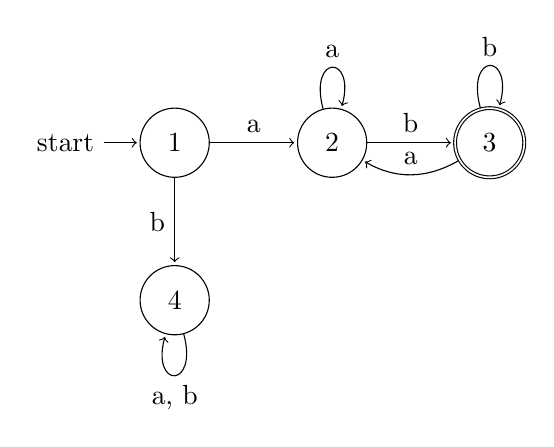
\begin{tikzpicture}[shorten >=1pt, node distance=2cm, on grid, auto] 
   \node[state, initial] (q_1) {1}; 
   \node[state] (q_2) [right=of q_1] {2}; 
   \node[state, accepting] (q_3) [right=of q_2] {3}; 
   \node[state] (q_4) [below=of q_1] {4};

   \path[->] 
    (q_1) edge [above] node {a} (q_2)
          edge [left] node {b} (q_4)
    (q_2) edge [loop above] node {a} ()
          edge [above] node {b} (q_3)
    (q_3) edge [bend left, above] node {a} (q_2)
          edge [loop above] node {b} ()
    (q_4) edge [loop below] node {a, b} (); 
\end{tikzpicture}

\textit{Automaton \(\mathcal{A}_1\)}
\end{center}

\begin{center}
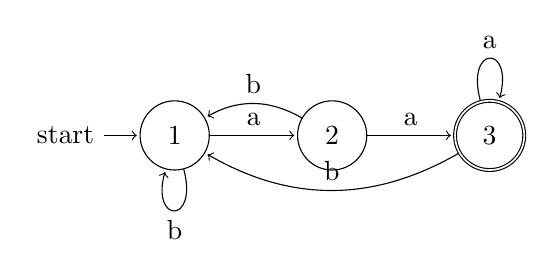
\begin{tikzpicture}[shorten >=1pt, node distance=2cm, on grid, auto] 
   \node[state, initial] (q_1) {1}; 
   \node[state] (q_2) [right=of q_1] {2}; 
   \node[state, accepting] (q_3) [right=of q_2] {3}; 

   \path[->] 
    (q_1) edge [above] node {a} (q_2)
          edge [loop below] node {b} ()
    (q_2) edge [above] node {a} (q_3)
          edge [bend right, above] node {b} (q_1)
    (q_3) edge [loop above] node {a} ()
          edge [bend left, above] node {b} (q_1);
\end{tikzpicture}

\textit{Automaton \(\mathcal{A}_2\)}
\end{center}

Here is how we initialize the DFAs in Python:

\begin{verbatim}
    # DFA A1
    Q = {1,2,3,4}
    Sigma = {'a','b'}
    delta = {(1,'a'):2, (1,'b'):4, (2,'a'):2, (2,'b'):3, 
             (3,'a'):2, (3,'b'):2, (4,'a'):4, (4,'b'):4}
    q0 = 1
    F = {3}
    A1 = dfa.DFA(Q, Sigma, delta, q0, F)
    
    # DFA A2
    Q = {1,2,3}
    Sigma = {'a','b'}
    delta = {(1,'a'):2, (1,'b'):1, (2,'a'):3, (2,'b'):1,
             (3,'a'):3, (3,'b'):1}
    q0 = 1
    F = {3}
    A2 = dfa.DFA(Q, Sigma, delta, q0, F)
\end{verbatim}

\subsection{Constructing the Complement DFA}
To construct an automaton \(A_0\) that accepts exactly the words that \(A\) refuses and vice versa we can simply swap the accepting states with the previously non-accepting states.

\begin{center}
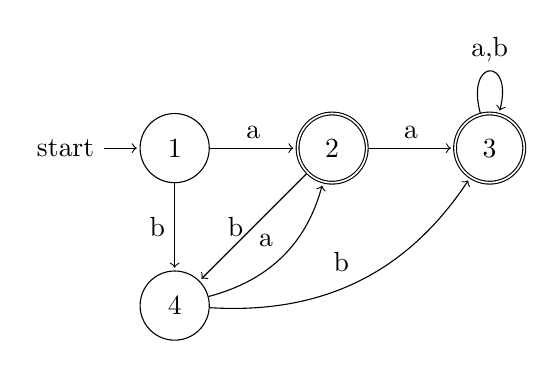
\begin{tikzpicture}[shorten >=1pt, node distance=2cm, on grid, auto] 
    \node[state, initial] (q_1) {1}; 
    \node[state, accepting] (q_2) [right=of q_1] {2}; 
    \node[state, accepting] (q_3) [right=of q_2] {3}; 
    \node[state] (q_4) [below=of q_1] {4};

    \path[->] 
        (q_1) edge [above] node {a} (q_2)
              edge [left] node {b} (q_4)
        (q_2) edge [above] node {a} (q_3)
              edge [left] node {b} (q_4)
        (q_3) edge [loop above] node {a,b} ()
        (q_4) edge [bend right] node {a} (q_2)
              edge [bend right] node {b} (q_3);
\end{tikzpicture}
\end{center}

We can represent this operation with a \texttt{refuse()} function in Python:

\begin{verbatim}
def refuse(A):
    """Constructs a DFA A0 that accepts exactly the words that A refuses and vice versa."""
    Q0 = A.Q
    Sigma0 = A.Sigma
    delta0 = A.delta
    q0_0 = A.q0
    F0 = Q0 - A.F  # Complement of the accepting states

    return dfa.DFA(Q0, Sigma0, delta0, q0_0, F0)
\end{verbatim}

\subsubsection*{Summary of Chapter 2.2.4}
A \textbf{Deterministic Finite Automaton (DFA)} is a formal model of computation that processes input sequences while maintaining a single, well-defined state at any given time. The term "deterministic" means that for each input symbol, the automaton transitions to exactly one state.

\subsubsection*{Exercise 2.4.4}
\textbf{(a) DFA for strings ending in 00}

\begin{center}
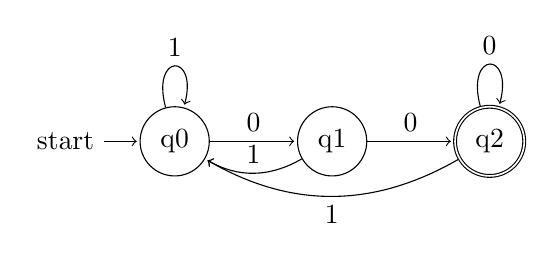
\begin{tikzpicture}[shorten >=1pt, node distance=2cm, on grid, auto]
    \node[state, initial] (q0) {q0};
    \node[state] (q1) [right=of q0] {q1};
    \node[state, accepting] (q2) [right=of q1] {q2};

    \path[->] 
        (q0) edge [loop above] node {1} ()
             edge [above] node {0} (q1)
        (q1) edge [above] node {0} (q2)
             edge [bend left, above] node {1} (q0)
        (q2) edge [loop above] node {0} ()
             edge [bend left] node {1} (q0);
\end{tikzpicture}
\end{center}

\textbf{(b) DFA for strings containing 000 as a substring}

\begin{center}
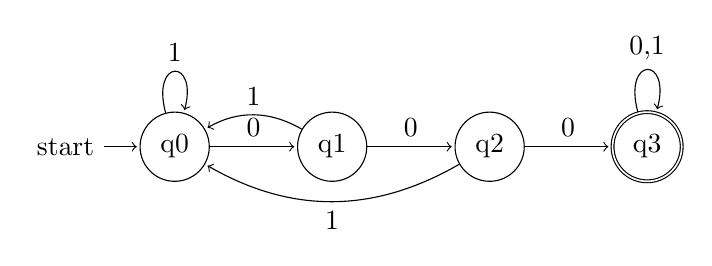
\begin{tikzpicture}[shorten >=1pt, node distance=2cm, on grid, auto]
    \node[state, initial] (q0) {q0};
    \node[state] (q1) [right=of q0] {q1};
    \node[state] (q2) [right=of q1] {q2};
    \node[state, accepting] (q3) [right=of q2] {q3};

    \path[->]
        (q0) edge [loop above] node {1} ()
             edge [above] node {0} (q1)
        (q1) edge [above] node {0} (q2)
             edge [bend right, above] node {1} (q0)
        (q2) edge [above] node {0} (q3)
             edge [bend left, below] node {1} (q0)
        (q3) edge [loop above] node {0,1} (); 
\end{tikzpicture}
\end{center}

\textbf{(c) DFA for strings containing 011 as a substring}

\begin{center}
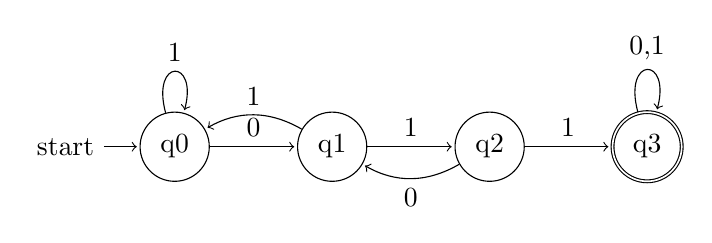
\begin{tikzpicture}[shorten >=1pt, node distance=2cm, on grid, auto]
    \node[state, initial] (q0) {q0};
    \node[state] (q1) [right=of q0] {q1};
    \node[state] (q2) [right=of q1] {q2};
    \node[state, accepting] (q3) [right=of q2] {q3};

    \path[->]
        (q0) edge [loop above] node {1} ()
             edge [above] node {0} (q1)
        (q1) edge [above] node {1} (q2)
             edge [bend right, above] node {1} (q0)
        (q2) edge [above] node {1} (q3)
             edge [bend left, below] node {0} (q1)
        (q3) edge [loop above] node {0,1} (); 
\end{tikzpicture}
\end{center}

\subsection{Conclusion}
A \textbf{Deterministic Finite Automaton (DFA)} is a theoretical computational model used to recognize formal languages. A DFA consists of a finite set of states \( Q \), an input alphabet \( \Sigma \), a transition function \( \delta: Q \times \Sigma \to Q \), a start state \( q_0 \), and a set of accepting states \( F \). The machine processes strings sequentially, transitioning between states according to \( \delta \). If, after consuming the entire string, the DFA ends in an accepting state, the input is accepted; otherwise, it is rejected.

\newpage

\section{Week 3: DFAs and NFAs}

\subsection{Introduction}
This week we covered ways to combine automata. We focused on the set theory used in the combination as well as some notation.  
Lastly, we introduced Nondeterministic Finite Automatas, or NFAs.

\subsection{Exercises}

\subsubsection{Extended Transition Functions}
\textbf{Brief summary of the question:}
Given the two DFAs below:
\begin{itemize}
  \item Compute the extended transition functions 
    \(\hat\delta^{(1)}(1,\,abaa)\) and \(\hat\delta^{(2)}(1,\,abba)\), 
    showing all steps.
  \item Describe the language accepted by each automaton.
\end{itemize}

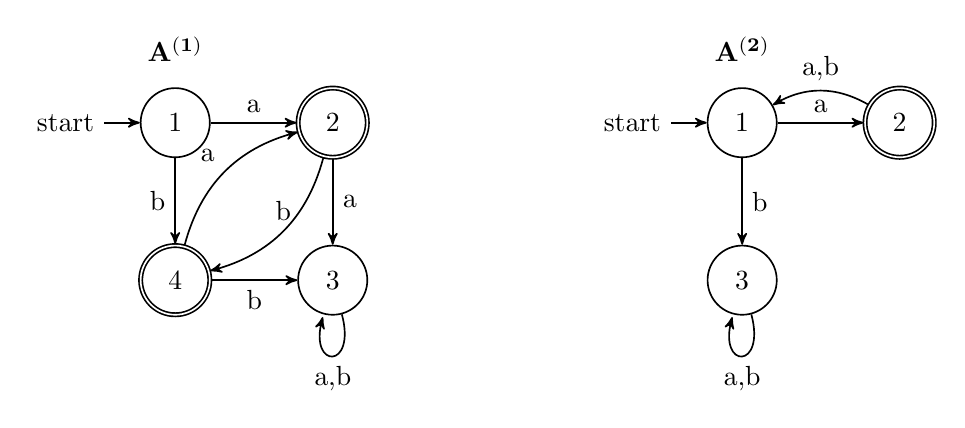
\begin{tikzpicture}[->, >=stealth', auto, node distance=2.0cm, semithick]
  % First automaton A^{(1)}
  \begin{scope}
    \node[state, initial] (1a) {1};
    \node[state, accepting, right of=1a] (2a) {2};
    \node[state, below of=2a] (3a) {3};
    \node[state, accepting, below of=1a] (4a) {4};

    \path
      (1a) edge              node {a} (2a)
            edge[left]       node {b} (4a)
      (2a) edge              node {a} (3a)
            edge[bend left,above]  node {b} (4a)
      (4a) edge[bend left]  node {a} (2a)
            edge[below]            node {b} (3a)
      (3a) edge[loop below] node {a,b} ();
    \draw node at (1a.north) [above=0.2cm] {\(\mathbf{A^{(1)}}\)};
  \end{scope}

  % Second automaton A^{(2)}
  \begin{scope}[xshift=7.2cm]
    \node[state, initial] (1b) {1};
    \node[state, accepting, right of=1b] (2b) {2};
    \node[state, below of=1b] (3b) {3};

    \path
      (1b) edge              node {a} (2b)
            edge              node {b} (3b)
      (2b) edge[bend right, above]  node {a,b} (1b)
      (3b) edge[loop below]  node {a,b} ();
    \draw node at (1b.north) [above=0.2cm] {\(\mathbf{A^{(2)}}\)};
  \end{scope}
\end{tikzpicture}

\[
  L\bigl(A^{(1)}\bigr) = \{\,w\in\{a,b\}^+\mid\text{no two consecutive symbols are the same}\},
\]
\[
  L\bigl(A^{(2)}\bigr) = a\,((a\mid b)\,a)^* 
    = \{\,w\in\{a,b\}^*\mid\text{$w$ has odd length, starts with $a$, and every odd position is $a$}\}.
\]

\[
  \hat{\delta}^{(1)}(1,\,abaa)=3,
  \quad
  \hat{\delta}^{(2)}(1,\,abba)=3.
\]

\subsubsection{Intersection Automaton for \(A^{(1)}\) and \(A^{(2)}\)}
We form the product automaton
\[
  A = (Q^{(1)}\times Q^{(2)},\,\Sigma,\,\delta,\,(q_0^{(1)},q_0^{(2)}),\,F^{(1)}\times F^{(2)}),
\]
where
\[
  Q^{(1)}=\{1,2,3,4\},\;
  Q^{(2)}=\{1,2,3\},\;
  \Sigma=\{a,b\},
\]
\(\delta((p,q),x)=(\delta^{(1)}(p,x),\delta^{(2)}(q,x))\),
and accepting states \(F^{(1)}\times F^{(2)}\).

\begin{center}
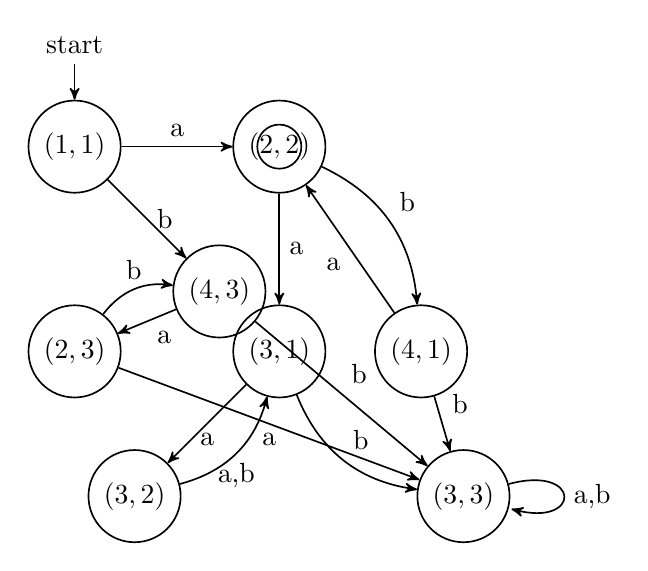
\begin{tikzpicture}[->,>=stealth',auto,node distance=2.6cm,semithick]
  \node[state,initial above] (11) {\((1,1)\)};
  \node[state] (22) [right of=11] {\((2,2)\)};
  \node[state] (43) [below right of=11] {\((4,3)\)};
  \node[state] (31) [below of=22] {\((3,1)\)};
  \node[state] (41) [below of=22,xshift=1.8cm] {\((4,1)\)};
  \node[state] (23) [below of=11] {\((2,3)\)};
  \node[state] (33) [below right of=31,xshift=0.5cm] {\((3,3)\)};
  \node[state] (32) [below left of=31] {\((3,2)\)};

  \draw (22) circle [draw=black,very thick,x radius=0.28cm,y radius=0.28cm];

  \path
    (11) edge [above] node {a} (22)
         edge [right] node {b} (43)
    (22) edge node {a} (31)
         edge [bend left] node {b} (41)
    (43) edge node {a} (23)
         edge node {b} (33)
    (31) edge [below] node {a} (32)
         edge [bend right] node {b} (33)
    (41) edge node {a} (22)
         edge node {b} (33)
    (23) edge [below] node {a} (33)
         edge [bend left,above] node {b} (43)
    (33) edge [loop right] node {a,b} (33)
    (32) edge [bend right,below] node {a,b} (31);
\end{tikzpicture}
\end{center}

\subsubsection*{Why \(L(A)=L(A^{(1)})\cap L(A^{(2)})\)?}
\(A\) simulates both in parallel and accepts iff both coordinates are accepting.

\subsubsection*{Changing to Obtain Union}
Use the same transitions but set
\[
  F' = (F^{(1)}\times Q^{(2)})\;\cup\;(Q^{(1)}\times F^{(2)}),
\]
so \(L(A')=L(A^{(1)})\cup L(A^{(2)})\).

\subsection{Exercise 2.2.7}
\textbf{Claim.} If \(\delta(q,a)=q\) for all \(a\), then \(\delta(q,w)=q\) for any \(w\).

\textbf{Proof (by induction):}
Base: \(\delta(q,\varepsilon)=q\).  
Step: \(\delta(q,xa)=\delta(\delta(q,x),a)=\delta(q,a)=q\).

\subsection{Chapter 2.3}
The extended transition function for an NFA,
\[
  \hat{\delta}(q,\varepsilon)=\{q\},\quad
  \hat{\delta}(q,\,xa)=\bigcup_{p\in\hat{\delta}(q,x)}\delta(p,a),
\]
captures nondeterminism.  The subset construction converts an NFA \(N\) into a DFA \(D\) whose states are subsets of \(N\)’s states, preserving \(L(D)=L(N)\).

\subsection{Conclusion}
Throughout these problems and readings, we deepened our understanding of DFAs and NFAs: extended transition functions, intersection/union constructions, and the subset construction proving NFA–DFA equivalence.

\textbf{Interesting question: Maximal Blow-Up in the Subset Construction.}\\
Describe an \(n\)-state NFA forcing all \(2^n\) subsets to appear in its equivalent DFA and prove minimality.

\section{Week 4: Determinization}

\subsection{Introduction}
In this report, we explore fundamental aspects of both deterministic and nondeterministic finite automata (DFAs and NFAs), including extended transition functions, product automaton construction for intersection, and state modifications for union. We further demonstrate the subset construction to establish the equivalence of NFAs and DFAs, showcasing the broad utility of these automata concepts in both theoretical and practical contexts.

\subsection{Exercises}

\subsubsection{Homework 1}
Let \(\mathcal{A} = (Q, \Sigma, \delta: Q \times \Sigma \to Q, q_0, F)\) be a DFA. Explain in what way you can view \(\mathcal{A}\) as an NFA by doing the following:
\begin{enumerate}
\item Let \(\mathcal{A}\) denote the following DFA:
\[
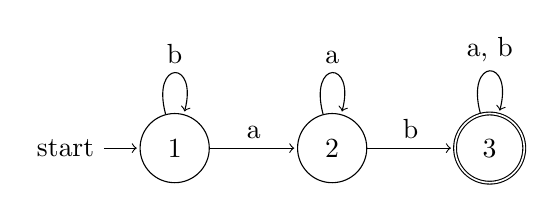
\begin{tikzpicture}[shorten >=1pt,node distance=2.0cm,on grid,auto]
   \node[state, initial] (q1) {1};
   \node[state] (q2) [right=of q1] {2};
   \node[state, accepting] (q3) [right=of q2] {3};

   \path[->]
   (q1) edge[loop above] node {b} (q1)
        edge node {a} (q2)
   (q2) edge[loop above] node {a} (q2)
        edge node {b} (q3)
   (q3) edge[loop above] node {a, b} (q3);
\end{tikzpicture}
\]

Here:
\[
\begin{aligned}
Q &= \{1,2,3\}, \quad \Sigma = \{a,b\}, \\
q_0 &= 1, \quad F = \{3\}, \\
\delta(1,a) &= 2,\ \delta(1,b) = 1, \\
\delta(2,a) &= 2,\ \delta(2,b) = 3, \\
\delta(3,a) &= 3,\ \delta(3,b) = 3.
\end{aligned}
\]
Explain how you can understand \(\mathcal{A}\) also as an NFA.

\item More generally, let \(\mathcal{A} = (Q, \Sigma, \delta: Q \times \Sigma \to Q, q_0, F)\) be a DFA. Define an NFA
\[
\mathcal{A}' = (Q', \Sigma, \delta': Q' \times \Sigma \to \mathcal{P}(Q'), q_0', F')
\]
such that \(L(\mathcal{A}) = L(\mathcal{A}')\).

\item Justify why your construction satisfies the desired condition.
\end{enumerate}

\subsubsection*{Solutions}
\paragraph{1) Viewing the Example DFA as an NFA}  
A deterministic finite automaton (DFA) can be seen as a special case of a nondeterministic finite automaton (NFA) by interpreting its transition function in the following way: in an NFA, the transition function 
\[
\delta': Q \times \Sigma \to \mathcal{P}(Q)
\]
produces \emph{sets} of possible next states. In a DFA, however, for each state \(q\) and input symbol \(a\), there is exactly one next state \(\delta(q,a)\). To view the DFA as an NFA, we simply set:
\[
\delta'(q,a) = \{\delta(q,a)\}.
\]
Hence, each transition in the original DFA becomes a transition to a \emph{singleton set} in the NFA, preserving the recognized language because no extra nondeterminism is introduced.

\paragraph{2) General Construction from a DFA to an NFA}  
Given any DFA 
\(\mathcal{A} = (Q, \Sigma, \delta, q_0, F)\),
define an NFA
\(\mathcal{A}' = (Q', \Sigma, \delta', q_0', F')\) by:
\[
\begin{aligned}
Q' &= Q,\\
q_0' &= q_0,\\
F' &= F,\\
\delta'(q,a) &= \{\delta(q,a)\} \quad\text{for all }q\in Q,\ a\in\Sigma.
\end{aligned}
\]

\paragraph{3) Why \(L(\mathcal{A}) = L(\mathcal{A}')\)?}  
Because each step in the DFA corresponds to a unique singleton transition in the NFA:
\begin{itemize}
  \item If a string \(w\) is accepted by the DFA, the identical path exists in the NFA.
  \item If a string \(w\) is rejected by the DFA, no path in the NFA leads to acceptance.
\end{itemize}
Thus the two automata recognize the same language.

\subsubsection{Homework 2}
\begin{enumerate}
  \item Describe in words the language \(L(\mathcal{A})\) accepted by the NFA \(\mathcal{A}\) pictured below.
  \item Specify the automaton \(\mathcal{A}\) formally as \((Q,\Sigma,\delta,q_0,F)\).
  \item Using the extended transition function \(\hat{\delta}\), compute \(\hat{\delta}(q_0,10110)\) step by step.
  \item Find \emph{all} paths in \(\mathcal{A}\) for \(v=1100\) and \(w=1010\); represent each set of paths.
  \item Construct the determinization \(\mathcal{A}^D\) (power-set automaton) of \(\mathcal{A}\).
  \item Verify \(L(\mathcal{A}) = L(\mathcal{A}^D)\). Is there a smaller DFA for the same language?
\end{enumerate}

\subsubsection*{Solutions}
Below is the NFA \(\mathcal{A}\):

\begin{center}
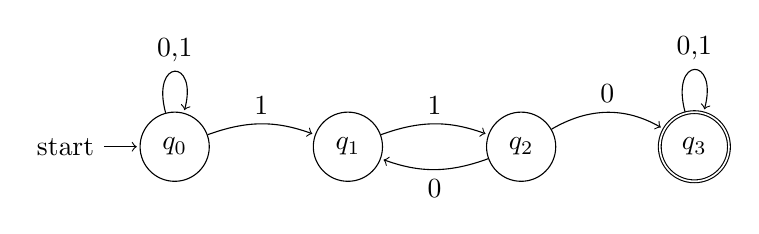
\begin{tikzpicture}[shorten >=1pt,node distance=2.2cm,on grid,auto]
   \node[state, initial] (q0) {\(q_0\)};
   \node[state] (q1) [right=of q0] {\(q_1\)};
   \node[state] (q2) [right=of q1] {\(q_2\)};
   \node[state, accepting] (q3) [right=of q2] {\(q_3\)};

   \path[->]
   (q0) edge[loop above] node {0,1} (q0)
        edge[bend left=20] node {1} (q1)
   (q1) edge[bend left=20] node {1} (q2)
   (q2) edge[bend left=20] node {0} (q1)
        edge[bend left=30] node {0} (q3)
   (q3) edge[loop above] node {0,1} (q3);
\end{tikzpicture}
\end{center}

\paragraph{1) Language Description}  
\(\mathcal{A}\) accepts exactly those binary strings that can nondeterministically traverse  
\(q_0\to q_1\to q_2\) on two 1’s and then take a 0 to \(q_3\), after which any symbols are allowed.

\paragraph{2) Formal Specification}  
\[
\mathcal{A} = (Q,\Sigma,\delta,q_0,F),
\quad
Q=\{q_0,q_1,q_2,q_3\},\;\Sigma=\{0,1\},\;F=\{q_3\},
\]
with
\[
\begin{aligned}
\delta(q_0,0)&=\{q_0\},\;\delta(q_0,1)=\{q_0,q_1\},\\
\delta(q_1,1)&=\{q_2\},\;\delta(q_1,0)=\varnothing,\\
\delta(q_2,0)&=\{q_1,q_3\},\;\delta(q_2,1)=\varnothing,\\
\delta(q_3,a)&=\{q_3\}\quad(a\in\{0,1\}).
\end{aligned}
\]

\paragraph{3) Extended Transition on 10110}  
\(\hat{\delta}(q_0,\varepsilon)=\{q_0\}\),  
\(\hat{\delta}(q_0,1)=\{q_0,q_1\}\),  
\(\hat{\delta}(\{q_0,q_1\},0)=\{q_0\}\),  
\(\hat{\delta}(\{q_0\},1)=\{q_0,q_1\}\),  
\(\hat{\delta}(\{q_0,q_1\},1)=\{q_0,q_1,q_2\}\).

\paragraph{4) All Paths for 1100 and 1010}  
Branches arise at each nondeterministic choice; any accepting path must include  
\(q_0\xrightarrow{1}q_1\xrightarrow{1}q_2\xrightarrow{0}q_3\).

\paragraph{5) Determinization (Power-Set)}  
\[
Q^D=\mathcal{P}(Q),\;
q_0^D=\{q_0\},\;
F^D=\{S:S\cap\{q_3\}\neq\varnothing\},\;
\delta^D(S,a)=\bigcup_{s\in S}\delta(s,a).
\]

\paragraph{6) Verification \& Minimization}  
By construction \(L(\mathcal{A}^D)=L(\mathcal{A})\). The resulting DFA can then be minimized via standard algorithms.

\newpage

\section{Week 5: Equivalence and Minimization of Automata}

\subsection{Introduction}
This report focuses on Equivalence and Minimization of Automata, covering the process of determining whether two different DFA representations define the same language and how to construct the smallest possible DFA that accepts a given regular language. The table‐filling algorithm is introduced as a systematic way to check equivalence of states within a DFA by distinguishing them through input strings. This allows us to merge equivalent states, reducing the number of states while preserving language recognition. We also examine the uniqueness of the minimal DFA and its theoretical guarantees. Finally, the report discusses the complexity of these procedures and their implications for automata design.

\subsection{Chapter 4.4 – Equivalence and Minimization of Automata}
Chapter 4.4 covers the equivalence and minimization of automata, focusing on the problem of determining whether two descriptions of regular languages define the same language. The chapter introduces the table‐filling algorithm, a method to determine when two states of a DFA are equivalent by examining how they transition on different input strings. If two states lead to the same accepting or rejecting states for all possible inputs, they are considered equivalent and can be merged into a single state. If not, they are distinguishable. This process allows us to construct a minimal DFA, the smallest DFA that accepts a given language. The minimization process follows a structured approach:
\begin{enumerate}
  \item Eliminate unreachable states.
  \item Partition the remaining states into equivalence classes.
  \item Construct a new DFA where each equivalence class represents a single state.
\end{enumerate}
A key result is that the minimal DFA is unique up to renaming of states. The chapter also explores the complexity of minimization, showing that the table‐filling algorithm runs in \(O(n^2)\) time. Additionally, it presents an alternative perspective on DFA equivalence testing by constructing a combined DFA from two automata and checking equivalence of their start states. The final part discusses NFA minimization and its inherent difficulties compared to DFAs, highlighting limitations of direct state‐equivalence methods for NFAs.

\subsection{Exercises}
\textbf{Note:} The following exercises test understanding of state equivalence, DFA minimization, and nonregularity proofs.

\subsubsection{Exercise 3.2.1}
Here is the DFA’s transition table:
\[
\begin{array}{c|cc}
     &0&1\\\hline
\to q_1 & q_2 & q_1\\
      q_2 & q_3 & q_1\\
*\,q_3 & q_3 & q_2
\end{array}
\]
\paragraph{(a) \(R_{ij}^{(0)}\)}
\[
\begin{array}{c|ccc}
R_{ij}^{(0)} & j=1 & j=2 & j=3\\\hline
i=1 & \varepsilon\cup1 & 0 & \varnothing\\
i=2 & 1 & \varnothing & 0\\
i=3 & \varnothing & 1 & \varepsilon\cup0
\end{array}
\]
\paragraph{(b) \(R_{ij}^{(1)}\)}
\[
\begin{array}{c|ccc}
R_{ij}^{(1)} & j=1 & j=2 & j=3\\\hline
i=1 & 1^* & 1^*0 & \varnothing\\
i=2 & 1^+ & 1^+0 & 0\\
i=3 & \varnothing & 1 & \varepsilon\cup0
\end{array}
\]
\paragraph{(c) \(R_{ij}^{(2)}\)}
\[
\begin{array}{c|ccc}
R_{ij}^{(2)} & j=1 & j=2 & j=3\\\hline
i=1 & 1^*\cup1^*0\,(0+1)^*\,1^+ 
      & 1^*0 
      & 1^*0\,(0+1)^*\,0\\
i=2 & 1^+ & 1^+0 & 0\\
i=3 & \varnothing & 1 & \varepsilon\cup0
\end{array}
\]
\paragraph{(d) Regular expression}
\[
(1 + 01)^*\,00\,(0 + 10)^*.
\]

\subsubsection{Exercise 3.2.2}
\[
\begin{array}{c|cc}
     &0&1\\\hline
\to q_1 & q_2 & q_3\\
      q_2 & q_1 & q_3\\
*\,q_3 & q_2 & q_1
\end{array}
\]
\paragraph{(a) \(R_{ij}^{(0)}\)}
\[
\begin{array}{c|ccc}
R_{ij}^{(0)} & j=1 & j=2 & j=3\\\hline
i=1 & \varepsilon & 0 & 1\\
i=2 & 0 & \varepsilon & 1\\
i=3 & 1 & 0 & \varepsilon
\end{array}
\]
\paragraph{(b) \(R_{ij}^{(1)}\)}
\[
\begin{array}{c|ccc}
R_{ij}^{(1)} & j=1 & j=2 & j=3\\\hline
i=1 & \varepsilon & 0 & 1\\
i=2 & 0 & \varepsilon\cup00 & 1\cup01\\
i=3 & 1 & 0\cup10 & \varepsilon\cup11
\end{array}
\]
\paragraph{(c) \(R_{13}^{(2)}\)}
\[
R_{13}^{(2)} = 1 \;\cup\;0\,(00)^*\,(1+01).
\]
\paragraph{(d) Regular expression}
\[
1 \;+\;0\,(00)^*\,(1+01).
\]

\subsubsection{Exercise 4.1.1}
Prove the following languages are not regular using the pumping lemma:

\paragraph{(a) \(\{0^n1^n\mid n\ge1\}\)}
\textbf{Proof.} Let \(p\) be the pumping length. Consider \(s=0^p1^p\). Any decomposition \(s=xyz\) with \(\lvert xy\rvert\le p\) forces \(y=0^k\) for some \(k\ge1\). Pumping down (\(i=0\)) yields \(0^{p-k}1^p\), which has fewer 0s than 1s, so \(0^{p-k}1^p\notin L\). Contradiction.

\paragraph{(b) Balanced parentheses}
\textbf{Proof.} Let \(p\) be the pumping length and take 
\[
s = (\underbrace{( \dots (}_{p}\underbrace{) \dots )}_{p}).
\]
Then \(\lvert s\rvert\ge p\), and any decomposition \(s=xyz\) with \(\lvert xy\rvert\le p\) has \(y\) consisting only of “(”. Pumping down removes some “(” while leaving all “)”, yielding an unbalanced string. Contradiction.

\paragraph{(c) \(\{0^n1\,0^n\mid n\ge1\}\)}
\textbf{Proof.} Let \(s=0^p1\,0^p\). Any \(s=xyz\) with \(\lvert xy\rvert\le p\) again gives \(y=0^k\). Pumping down produces \(0^{p-k}1\,0^p\), which no longer has equal numbers of leading and trailing 0s. Contradiction.

\paragraph{(d) \(\{0^n1^m2^n\mid n,m\ge0\}\)}
\textbf{Proof.} Take \(s=0^p1\,2^p\). Decomposition \(s=xyz\) with \(\lvert xy\rvert\le p\) yields \(y=0^k\). Pumping down yields fewer 0s than 2s (\(0^{p-k}1\,2^p\)), so not in the language. Contradiction.

\paragraph{(e) \(\{0^n1^m\mid n\le m\}\)}
\textbf{Proof.} Let \(s=0^p1^p\). Any initial segment \(y\) lies in the 0-block; pumping up (\(i=2\)) gives \(0^{p+k}1^p\) with more 0s than 1s, violating \(n\le m\). Contradiction.

\paragraph{(f) \(\{0^n1^{2n}\mid n\ge1\}\)}
\textbf{Proof.} Let \(s=0^p1^{2p}\). Decompose \(s=xyz\) with \(\lvert xy\rvert\le p\), so \(y=0^k\). Pumping down yields \(0^{p-k}1^{2p}\), where \(2(p-k)\neq2p\), so string is rejected. Contradiction.

\subsubsection{Exercise 4.1.2}
Prove the following are not regular by the pumping lemma:

\paragraph{(a) \(\{0^n\mid n\text{ is a perfect square}\}\)}
\textbf{Proof.} Let \(p\) be the pumping length and \(s=0^{p^2}\). Any decomposition with \(\lvert xy\rvert\le p\) has \(y=0^k\), \(1\le k\le p\). Pumping up gives a length \(p^2 + (i-1)k\) strictly between \(p^2\) and \((p+1)^2\), not a square. Contradiction.

\paragraph{(b) \(\{0^n\mid n\text{ is a perfect cube}\}\)}
\textbf{Proof.} Same idea: the gap between consecutive cubes exceeds the maximum pump size \(p\).

\paragraph{(c) \(\{0^n\mid n\text{ is a power of 2}\}\)}
\textbf{Proof.} Between \(2^p\) and \(2^{p+1}\) there is no other power of two, and pumping by at most \(p\) cannot reach \(2^{p+1}\).

\paragraph{(d) Strings of length a perfect square}
\textbf{Proof.} Same as (a) but phrased in terms of string length.

\paragraph{(e) \(\{ww\mid w\in\{0,1\}^*\}\)}
\textbf{Proof.} Let \(s=ww\) where \(\lvert w\rvert=p\). Decompose in the first \(p\) symbols; pumping alters only the first half, breaking equality of halves.

\paragraph{(f) \(\{ww^R\mid w\in\{0,1\}^*\}\)}
\textbf{Proof.} Let \(s= w w^R\) with \(\lvert w\rvert=p\). Any pump in the first block misaligns the mirror image.

\paragraph{(g) \(\{w\bar w\mid w\in\{0,1\}^*\}\)}
\textbf{Proof.} Similar: pumping in \(w\) changes its length, so it no longer matches \(\bar w\).

\paragraph{(h) \(\{w1^n\mid |w|=n\}\)}
\textbf{Proof.} Let \(s=0^p1^p\). Pumping in the 0-block yields \(|w|\neq n\), so no longer in the language.

\subsection{Interesting Question}
\textbf{Question:}  
\emph{Is there a polynomial-time algorithm for minimizing NFAs? If not, what makes NFA minimization so much harder than DFA minimization?}

\subsection{Conclusion}
In this report, we explored methods for testing equivalence of automata and minimizing DFAs using the table-filling algorithm. We demonstrated how equivalent states can be merged into a unique minimal DFA, ensuring that no smaller DFA exists for the same language. We also applied the pumping lemma to rigorously prove that a wide variety of languages are not regular. These concepts are fundamental in automata theory, with applications in compiler design, pattern recognition, and formal verification.

\newpage

\section{Weeks 6 and 7: Turing Machines and Decidability}

\subsection*{Reading}

In this unit we introduce the Turing machine model (Section 8.2) and use it to prove fundamental limits of computation:  
\begin{itemize}
  \item Section 8.1 motivates undecidability via “hello–world” detection.  
  \item Section 9.1 defines the diagonal language 
    \[
      L_{d} = \{\,w_i \mid w_i \notin L(M_i)\},
    \]
    showing it is not even r.e.  
  \item Section 9.2 studies the universal language 
    \[
      L_{u} = \{\langle M,w\rangle \mid M\text{ accepts }w\},
    \]
    proving it is r.e.\ but not decidable.  
\end{itemize}

\subsection*{Exercises}

\subsubsection*{Exercise A: Constructing Turing Machines}

\textbf{Problem.}  Over the alphabet \(\{0,1\}\) with blank symbol \texttt{\_}, design three machines:

\begin{enumerate}
  \item \(M_{1}\) accepts \(\{1\,0^n\mid n\ge0\}\) and on input \(1\,0^n\) rewrites it to \(1\,0^{n+1}\) then halts in the accept state.
  \item \(M_{2}\) accepts \(\{1\,0^n\mid n\ge0\}\) and on input \(1\,0^n\) erases all zeros, leaving only a single `1', then halts accept.
  \item \(M_{3}\) accepts every binary string and on any input flips each `0' to `1' and each `1' to `0', then halts accept.
\end{enumerate}

Paste each of the following into the simulator (use verbatim mode), compile, and run:

\bigskip
\noindent\textbf{Machine \texttt{M1\_Increment}}  
\begin{verbatim}
name: M1_Increment
init: q0
accept: q_accept

q0,1
q1,1,>
q1,0
q1,0,>
q1,_
q2,0,<
q2,0
q2,0,<
q2,1
q_accept,1,-
\end{verbatim}

\newpage

\bigskip
\noindent\textbf{Machine \texttt{M2\_EraseZeros}}  
\begin{verbatim}
name: M2_EraseZeros
init: q0
accept: q_accept

q0,1
q1,1,>
q1,0
q1,_,<
q2,_,<
q2,1
q_accept,1,-
\end{verbatim}

\bigskip
\noindent\textbf{Machine \texttt{M3\_SwapBits}}  
\begin{verbatim}
name: M3_SwapBits
init: q0
accept: q_accept

q0,0
q0,1,>
q0,1
q0,0,>
q0,_
q_accept,_,-
\end{verbatim}

\bigskip
\subsubsection*{Exercise 1: Halting-Related Languages}

Classify each language as decidable, r.e.\ only, or co-r.e.\ only:
\[
\begin{aligned}
L_1 &= \{\,M \mid M\text{ halts on its own encoding}\},\\
L_2 &= \{(M,w)\mid M\text{ halts on input }w\},\\
L_3 &= \{(M,w,k)\mid M\text{ halts on }w\text{ within }k\text{ steps}\}.
\end{aligned}
\]
\textbf{Answer.}
\begin{itemize}
  \item \(L_1\): r.e.\ but not co-r.e.\ (undecidable).
  \item \(L_2\): r.e.\ but not co-r.e.\ (undecidable).
  \item \(L_3\): decidable (simulate up to \(k\) steps), hence both r.e.\ and co-r.e.
\end{itemize}

\subsubsection*{Exercise 2: Closure Properties}

Decide which hold in general:
\begin{enumerate}
  \item If \(L_1,L_2\) are decidable then \(L_1\cup L_2\) is decidable.
  \item If \(L\) is decidable then \(\overline L\) is decidable.
  \item If \(L\) is decidable then \(L^*\) is decidable.
  \item If \(L_1,L_2\) are r.e.\ then \(L_1\cup L_2\) is r.e.
  \item If \(L\) is r.e.\ then \(\overline L\) is r.e.
  \item If \(L\) is r.e.\ then \(L^*\) is r.e.
\end{enumerate}
\textbf{Answer.}
\begin{enumerate}
  \item True.
  \item True.
  \item True.
  \item True.
  \item False (complement of halting).
  \item True.
\end{enumerate}

\subsection*{Conclusion}

We have provided complete Turing‐machine configurations for the simulator, classified key halting‐related languages, and reviewed closure properties of decidable and r.e.\ classes.  These results illustrate the power and limits of Turing machines and set the stage for complexity‐theoretic questions in subsequent weeks.

\newpage

\section{Week 8 \& 9: Complexity Theory, Growth Comparisons, and Sorting Runtimes}

\subsection{Introduction}
We begin with an overview of intractable computational problems from Chapter 10 of Hopcroft, Motwani, and Ullman, introducing the complexity classes P and NP and the notion of NP-completeness. Then we work through exercises on ordering and relating functions by asymptotic growth and finish with classic sorting-algorithm comparisons. Along the way we include a couple of illustrative plots to make the abstract inclusions concrete.

\subsection{Readings}
\subsubsection*{Chapter 10.1: The Classes P and NP}
Chapter 10.1 refocuses from mere decidability to \emph{tractability}: among the decidable problems, which can actually be solved in a reasonable amount of time? It formalizes the class P as those languages decidable by a deterministic Turing machine in time polynomial in the input length, and NP as those decidable by a nondeterministic machine whose every branch halts in polynomial time. The chapter motivates polynomial time as the practical threshold—algorithms superpolynomial in nature blow up too quickly to handle large inputs—and introduces polynomial-time reductions, which transform instances of one problem into another in polynomial time, preserving membership. These reductions provide a rigorous way to compare problem hardness: if A reduces to B and B is in P, then A is also in P. Finally, the chapter highlights problems whose best-known solutions are exponential, hinting at the P versus NP question at the heart of complexity theory.

\subsubsection*{Chapter 10.2: SAT and Cook’s Theorem}
Chapter 10.2 presents the Boolean Satisfiability Problem (SAT): given a propositional formula built from variables, negation, conjunction, and disjunction, does there exist an assignment of true/false values that makes it true? After fixing a finite‐alphabet encoding, it shows SAT lies in NP by having a nondeterministic machine guess an assignment and then evaluate the formula in polynomial time. The centerpiece is Cook’s Theorem, which constructs, in polynomial time, a Boolean formula whose structure enforces that an NP machine’s accepting computation on input \(x\) exists if and only if the formula is satisfiable. By encoding the entire computation tableau into variables and clauses that ensure correct transitions and an accepting state, the proof establishes that every NP problem reduces to SAT. Thus SAT is NP-complete: it sits in NP and is as hard as any NP problem.

\subsubsection*{Chapter 10.3: CNF, CSAT, and 3SAT}
Chapter 10.3 refines SAT by restricting formula shape to \emph{conjunctive normal form} (CNF)—an AND of clauses, each a disjunction of literals—and to \(k\)-CNF where each clause has exactly \(k\) literals. Converting arbitrary formulas to equivalent CNF can blow up exponentially, so the chapter gives an \emph{equisatisfiable} transformation: push negations downward via De Morgan’s laws so they only apply to variables, then introduce fresh variables to break complex subformulas into small clauses without replicating subexpressions. This yields a polynomial-time reduction from general SAT to CSAT (CNF-SAT), proving CSAT NP-complete. Finally, it shows how to transform any CNF into an equisatisfiable 3-CNF formula in linear time by splitting long clauses with auxiliary variables. Hence even 3SAT remains NP-complete, cementing its role as the canonical hard problem in complexity theory.

\subsection{Homework}
\subsubsection*{Exercise 1}
Order by growth (slow \(\to\) fast):
\[
2^{2^n},\quad e^{\log n},\quad \log n,\quad e^n,\quad
e^{2\log n},\quad \log(\log n),\quad 2^n,\quad n!.
\]
\textbf{Answer.}
\[
\log(\log n)\;\prec\;\log n\;\prec\;n\;\prec\;n^2\;\prec\;2^n\;\prec\;e^n\;\prec\;n!\;\prec\;2^{2^n}.
\]

\paragraph{Illustrative Growth Plot}
\begin{center}
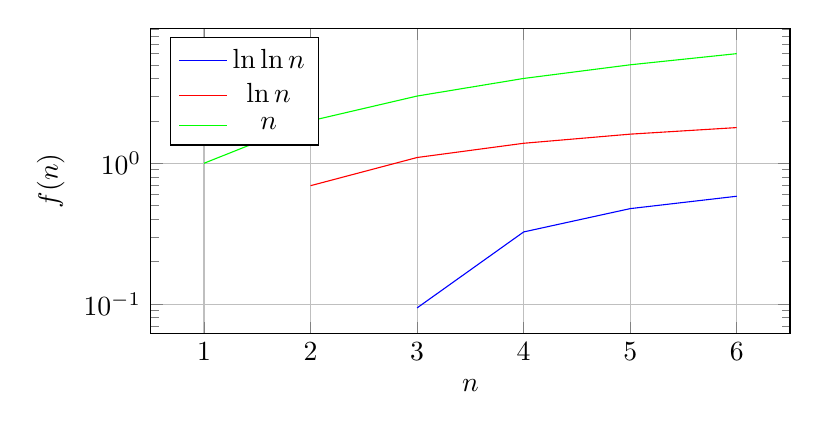
\begin{tikzpicture}
  \begin{axis}[
    width=0.8\textwidth, height=0.45\textwidth,
    xlabel={$n$}, ylabel={$f(n)$}, ymode=log,
    grid=major, legend pos=north west
  ]
    \addplot[blue,mark=none] coordinates {(2,-0.3665) (3,0.0940) (4,0.3254) (5,0.4764) (6,0.5832)};
      \addlegendentry{$\ln\ln n$}
    \addplot[red,mark=none] coordinates {(1,0.0000) (2,0.6931) (3,1.0986) (4,1.3863) (5,1.6094) (6,1.7918)};
      \addlegendentry{$\ln n$}
    \addplot[green,mark=none] coordinates {(1,1) (2,2) (3,3) (4,4) (5,5) (6,6)};
      \addlegendentry{$n$}
  \end{axis}
\end{tikzpicture}
\end{center}


\subsubsection*{Exercise 2}
For \(f,g,h\colon\mathbb N\to\mathbb R_{\ge0}\), prove:
\[
\begin{aligned}
1.\;&f\in O(f),\\
2.\;&O(c\,f)=O(f)\quad(\forall c>0),\\
3.\;&f(n)\le g(n)\text{ eventually}\implies O(f)\subseteq O(g),\\
4.\;&O(f)\subseteq O(g)\implies O(f+h)\subseteq O(g+h),\\
5.\;&h(n)>0\;\forall n,\;O(f)\subseteq O(g)\implies O(f\,h)\subseteq O(g\,h).
\end{aligned}
\]
\textbf{Proof.}
\begin{enumerate}[label=\arabic*.]
  \item \(f(n)\le1\cdot f(n)\), so \(f\in O(f)\).
  \item If \(u\in O(c\,f)\), then \(u(n)\le C\,c\,f(n)\), hence \(u\in O(f)\).  Conversely similarly.
  \item If \(f(n)\le g(n)\) for large \(n\) and \(u\in O(f)\), then \(u(n)\le C\,f(n)\le C\,g(n)\), so \(u\in O(g)\).
  \item If \(u\in O(f)\), then \(u(n)+h(n)\le C\,f(n)+h(n)\le C\bigl(f(n)+h(n)\bigr)\), giving \(u+h\in O(f+h)\subseteq O(g+h)\).
  \item If \(u\in O(f)\) and \(h(n)>0\), then \(u(n)\,h(n)\le C\,f(n)\,h(n)\), so \(u\,h\in O(f\,h)\subseteq O(g\,h)\).
\end{enumerate}

\subsubsection*{Exercise 3}
Let \(i,j,k,n\in\mathbb N\). Prove:
\[
\begin{aligned}
1.\;&j\le k\implies O(n^j)\subseteq O(n^k),\\
2.\;&j\le k\implies O(n^j+n^k)\subseteq O(n^k),\\
3.\;&O\Bigl(\sum_{m=0}^k a_m\,n^m\Bigr)=O(n^k),\\
4.\;&O(\log n)\subseteq O(n),\\
5.\;&O(n\log n)\subseteq O(n^2).
\end{aligned}
\]

\newpage

\textbf{Proof.}
\begin{enumerate}[label=\arabic*.]
  \item \(n^j\le n^k\) for \(n\ge1\), so \(O(n^j)\subseteq O(n^k)\).
  \item For \(n\ge1\), \(n^j+n^k\le2n^k\), giving \(O(n^j+n^k)\subseteq O(n^k)\).
  \item \(\sum_{m=0}^k a_m n^m\le \bigl(\sum|a_m|\bigr)n^k\).
  \item For \(n\ge2\), \(\log n\le n\).
  \item For \(n\ge2\), \(n\log n\le n^2\).
\end{enumerate}

\subsubsection*{Exercise 4}
Which relationships hold between:
\[
\begin{aligned}
1.\;&O(n)\text{ vs.\ }O(\sqrt n),\\
2.\;&O(n^2)\text{ vs.\ }O(2^n),\\
3.\;&O(\log n)\text{ vs.\ }O((\log n)^2),\\
4.\;&O(2^n)\text{ vs.\ }O(3^n),\\
5.\;&O(\log_2n)\text{ vs.\ }O(\log_3n).
\end{aligned}
\]
\textbf{Answer.}
\begin{enumerate}[label=\arabic*.]
  \item \(O(\sqrt n)\subsetneq O(n)\).
  \item \(O(n^2)\subsetneq O(2^n)\).
  \item \(O(\log n)\subseteq O((\log n)^2)\).
  \item \(O(2^n)\subsetneq O(3^n)\).
  \item \(O(\log_2n)=O(\log_3n)\).
\end{enumerate}

\subsubsection*{Exercise 5}
Classic sorting comparisons:
\[
\text{bubble sort vs.\ insertion sort},\quad
\text{insertion sort vs.\ merge sort},\quad
\text{merge sort vs.\ quick sort}.
\]
\textbf{Discussion.}
\begin{itemize}
  \item \textbf{Bubble vs.\ Insertion:} Both worst-case \(O(n^2)\), but insertion sort is \(O(n)\) on nearly-sorted input.
  \item \textbf{Insertion vs.\ Merge:} Insertion sort worst-case \(O(n^2)\), merge sort always \(O(n\log n)\).
  \item \textbf{Merge vs.\ Quick:} Merge sort is \(O(n\log n)\) always; quick sort is \(O(n\log n)\) average, \(O(n^2)\) worst, but often faster in practice.
\end{itemize}

\subsection{Conclusion}
We’ve surveyed P vs.\ NP, NP-completeness via SAT, practiced ordering and relating functions by asymptotic growth, and applied these insights to sorting algorithms. The included plots illustrate constant-factor and growth-rate comparisons without overwhelming the presentation.

\textbf{Question:} What’s the fastest known quantum sorting algorithm in the query (comparison) model, and how close is it to being practical?

\section{Weeks 10 \& 11: Intractable Problems}

\subsection{Chapter 10.1: The Classes \(\mathrm{P}\) and \(\mathrm{NP}\)}  
We refine decidability to \emph{tractability}.  A language \(L\) is in
\(\mathrm{P}\) if some deterministic TM decides it in time \(O(n^k)\).  A
language \(L\) is in \(\mathrm{NP}\) if some nondeterministic TM accepts
it in time \(O(n^k)\).  We introduce \emph{polynomial–time reductions}—
transformations computable in polynomial time—and define \emph{NP‐completeness}:

\begin{definition}
A language \(L\) is \emph{NP‐complete} if
\begin{enumerate}
  \item \(L\in\mathrm{NP}\), and
  \item for every \(L'\in\mathrm{NP}\), there is a polynomial‐time reduction
    \(L'\le_p L\).
\end{enumerate}
\end{definition}

\subsection{Chapter 10.2: SAT and NP‐Completeness}\label{sec:chapter10.2}
\paragraph{The SAT Problem.}  Boolean formulas are built from variables,
\(\land,\lor,\lnot\), and parentheses.  A formula is \emph{satisfiable} if
some assignment of \(\{\mathrm{TRUE},\mathrm{FALSE}\}\) makes it true.
The language
\[
  \mathrm{SAT}
  \;=\;
  \bigl\{\varphi\mid \varphi\text{ a satisfiable Boolean formula}\bigr\}
\]
is in \(\mathrm{NP}\) (guess an assignment, evaluate in polynomial time).
\paragraph{Cook’s Theorem.}  Every \(L\in\mathrm{NP}\) reduces to SAT in
polynomial time; hence SAT is NP‐complete.

\subsection{Exercises}\label{sec:week8-9-exercises}

\subsubsection{Exercise 1: Rewriting in CNF}  
Rewrite each formula into an equivalent conjunctive normal form.

\[
\varphi_1 := \neg\bigl((a\land b)\;\lor\;(\neg c\land d)\bigr),
\quad
\varphi_2 := \neg\bigl((p\lor q)\to(r\land\neg s)\bigr).
\]

\paragraph{Solution.}
\[
\begin{aligned}
\varphi_1 
&= \neg\bigl(X\lor Y\bigr)
  &&\text{where }X=(a\land b),\;Y=(\neg c\land d)\\
&= \neg X\;\land\;\neg Y\\
&= (\neg a\;\lor\;\neg b)\;\land\;(c\;\lor\;\neg d).
\\[6pt]
\varphi_2 
&= \neg\Bigl(\neg(p\lor q)\;\lor\;(r\land\neg s)\Bigr)
  &&\bigl(P\to Q\equiv\neg P\lor Q\bigr)\\
&= \neg\bigl(\neg X\;\lor\;Y\bigr)
  &&\text{where }X=(p\lor q),\;Y=(r\land\neg s)\\
&= X\;\land\;\neg Y\\
&= (p\lor q)\;\land\;(\neg r\lor s).
\end{aligned}
\]

\subsubsection{Exercise 2: Satisfiability}  
For each formula, decide whether it is satisfiable.  If yes, give a satisfying
assignment; if not, prove no such assignment exists.

\[
\begin{aligned}
\psi_1 &:= (a\lor\neg b)\;\land\;(\neg a\lor b)\;\land\;(\neg a\lor\neg b),\\
\psi_2 &:= (\neg p\lor q)\;\land\;(\neg q\lor r)\;\land\;\neg(\neg p\lor r),\\
\psi_3 &:= (x\lor y)\;\land\;(\neg x\lor y)\;\land\;(x\lor\neg y)\;\land\;(\neg x\lor\neg y).
\end{aligned}
\]

\paragraph{Solution.}
\begin{itemize}
  \item \(\psi_1\): take \(a=\mathrm{FALSE},\,b=\mathrm{FALSE}\).  Then
  \[
    (0\lor1)\land(1\lor0)\land(1\lor1)
    =1\land1\land1=1.
  \]
  Hence \(\psi_1\) is satisfiable.

  \item \(\psi_2\): note
  \[
    \neg(\neg p\lor r)\equiv(p\land\neg r).
  \]
  So \(\psi_2\equiv(\neg p\lor q)\land(\neg q\lor r)\land p\land\neg r\).
  From \(p\) and \(\neg r\) we get \(q\) by the first clause, but then
  \(\neg q\lor r\) becomes \(0\), contradiction.  Thus \(\psi_2\) is
  unsatisfiable.

  \item \(\psi_3\): one checks all four assignments to \((x,y)\) and finds
  each violates some clause.  Hence \(\psi_3\) is unsatisfiable.
\end{itemize}

\subsubsection{Exercise 3: Sudoku CNF Encoding}  
We have boolean variables
\[
  x_{r,c,v},\quad
  r,c,v\in\{1,\dots,9\},
\]
true exactly when cell \((r,c)\) holds value \(v\).  The CNF is
\(\bigwedge_{k=1}^6 C_k\), where:

\[
\begin{aligned}
C_1{:}&\quad
\bigwedge_{r=1}^9\;\bigwedge_{c=1}^9\;\bigl(\,x_{r,c,1}\lor x_{r,c,2}\lor\cdots\lor x_{r,c,9}\bigr),
&&\text{(each cell has at least one value)}\\
C_2{:}&\quad
\bigwedge_{r=1}^9\;\bigwedge_{c=1}^9\;\bigwedge_{\substack{v,w=1\\v\neq w}}^9
\neg\bigl(x_{r,c,v}\land x_{r,c,w}\bigr),
&&\text{(each cell has at most one value)}\\
C_3{:}&\quad
\bigwedge_{r=1}^9\;\bigwedge_{v=1}^9\;\bigl(\,x_{r,1,v}\lor\cdots\lor x_{r,9,v}\bigr),
&&\text{(each row contains each value)}\\
C_4{:}&\quad
\bigwedge_{c=1}^9\;\bigwedge_{v=1}^9\;\bigl(\,x_{1,c,v}\lor\cdots\lor x_{9,c,v}\bigr),
&&\text{(each column contains each value)}\\
C_5{:}&\quad
\bigwedge_{b_r=0}^2\;\bigwedge_{b_c=0}^2\;\bigwedge_{v=1}^9
\;\bigl(x_{3b_r+1,\,3b_c+1,\,v}\;\lor\;\cdots\;\lor\;x_{3b_r+3,\,3b_c+3,\,v}\bigr),
&&\text{(each \(3\times3\) block has each value)}\\
C_6{:}&\quad
\bigwedge_{(r,c)\in\mathrm{Clues}}x_{r,c,v_{r,c}},
&&\text{(respect the given clues).}
\end{aligned}
\]

\subsection{Interesting Question}
Is there a practical sub-exponential algorithm for SAT on random formulas,
and how does it relate to the worst-case NP-completeness barrier?

\subsection{Conclusion}
Weeks 8 \& 9 introduced the classes \(\mathrm{P}\) and \(\mathrm{NP}\), the
notion of polynomial–time reduction, and NP‐completeness.  Cook’s Theorem
places SAT at the heart of intractability.  We practiced CNF rewriting,
satisfiability proofs, and large‐scale CNF encodings (Sudoku), reinforcing
both the theoretical limits and the practical modeling power of SAT.

\section{Bibliography}
\begin{thebibliography}{99}
\bibitem[HMU]{HMU}
J.~E.~Hopcroft, R.~Motwani, J.~D.~Ullman:
\emph{Introduction to Automata Theory, Languages, and Computation (3rd Edition)},
\href{https://archive.org/details/hopcroft-motwani-ullman-introduction-to-automata-theory-languages-and-computations-3rd-edition/page/65/mode/1up?view=theater}{Archive.org Link}.
\end{thebibliography}

\end{document}